%---------- Terceiro Capitulo ----------
\chapter{Visão geral da área}\label{cha:visaogeral}

As inovações e evoluções em hardware e software dos dispositivos móveis têm atraído atenção de diversos tipos de pessoas, desde usuários leigos que utilizam poucas funcionalidades desses aparelhos aos pesquisadores que utilizam e se beneficiam da mobilidade e da robustez desses novos dispositivos em parte de seus projetos.

\section{Conectividade}
Os dispositivos móveis encontrados no mercado possibilitam que o usuário possam conectá-lo à Internet de alguma forma, sempre utilizando alguma tecnologia de comunicação sem fio, sendo que as mais comuns são as redes locais sem fio \sigla{WLAN}{Wireless Local Area Network} (\textit{Wireless Local Area Network}) e as redes de telefonia móvel (Celular).
\subsection{WLAN}
Ultimamente o uso da tecnologia de conexão à rede sem fios espalhou-se por todos os lugares, em casa, na universidade, no trabalho, nos aeroportos, hoteis, até em alguns restaurantes.
As redes sem fio são conhecidas como redes Wi-Fi, elas abrangem as tecnologias 802.11 do padrão \sigla{IEEE}{Institute of Electrical and Electronics Engineers} (\textit{Institute of Electrical and Electronics Engineers}).
\begin{citacao}
Wi-Fi é o nome associado à família do padrão IEEE 802.11\footnote{ieee802.org/11/index.shtml}. Assim como o
padrão 802.15, esse padrão opera em faixas de freqüências que não necessitam de licença para instalação e operação. Suas faixas de freqüência são 2,4GHz, 3,6GHz e 5GHz. As aplicações do padrão 802.11 diferem do padrão 802.15 quanto à utilização da rede e a mobilidade do usuário. Wi-Fi oferece alta potência de transmissão e cobre distâncias maiores, oferecendo redes sem fio locais (WLAN). \cite{vanni09}
\end{citacao}
Uma das maiores vantagens das redes Wi-Fi é a sua compatibilidade com praticamente todos os sistemas operacionais, incluindo dipositivos como impressoras e video-games.

As redes Wi-Fi fazem o uso das ondas de rádio para transmitir informações e os dispositivos devem ter um adaptador que traduzem os dados em sinais de rádio. Esses sinais são transmitidos através de uma antena para um decodificador conhecido como roteador, que decodifica os sinais e envia os dados para a Internet através de uma conexão com fios à rede \sigla{LAN}{Local Area Network} (\textit{Local Area Network}).

Como as redes sem fio funcionam recebendo e emitindo sinais, os dados recebidos da Internet são codificados em sinais de rádio pelo roteador e recebidos pelo adaptador do dispositivo conectado como pode ser visto na Figura \ref{fig:wlan}.
Os pontos de acesso às redes Wi-Fi podem ser públicas, como por exemplo nos aeroportos e restaurantes ou fechadas, como nos locais de trabalho e nas casas.

\begin{figure}[!htb]
	\centering
	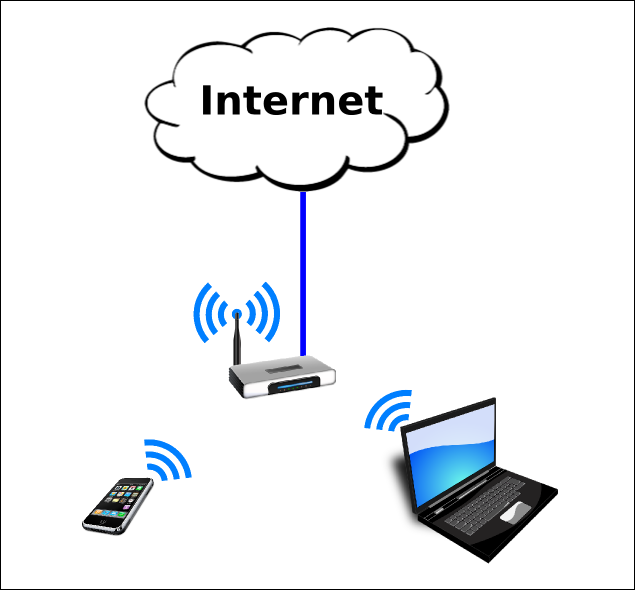
\includegraphics[width=0.45\textwidth]{wlan.png} % <- formatos PNG, JPG e PDF
	\caption[Organização de uma WLAN]{Organização de uma WLAN.}
	\label{fig:wlan}
\end{figure}

Pelo fato de não ser necessário ter acesso físico aos pontos de acesso, qualquer dispositivo com adaptador para redes sem fio poderia ter acesso à Internet através de qualquer roteador Wi-Fi que estivesse no seu alcance. Para bloquear esse acesso às redes Wi-Fi são utilizadas diversas tecnicas de autenticação com protocolos de criptografia como por exemplo:
\begin{itemize}
  \item \sigla{WEP}{Wired Equivalent Privacy} (\textit{Wired Equivalent Privacy})
  - É um algoritmo de segurança que foi introduzido originalmente como parte do protocolo 802.11 que garantiria a confidencialidade dos dados na rede Wi-Fi, mas infelizmente era um algoritmo fácil de quebrar, assim no ano de 2003 a \textit{Wi-Fi Alliance} \footnote{Uma associação da indústria global sem fins lucrativos. wi-fi.org/who-we-are} declarou que o WEP havia sido superado pelo WPA.
  \item \sigla{WPA}{Wi-Fi Protected Access} (\textit{Wi-Fi Protected Access})
  - O WPA e o \sigla{WPA2}{Wi-Fi Protected Access II} (\textit{Wi-Fi Protected Access II}) são dois protocolos de segurança e programas de certificação de segurança desenvolvidos pela \textit{Wi-Fi Alliance} para proteger redes de computadores sem fio. Foram desenvolvidos em resposta às graves deficiências encontradas por pesquisadores no sistema anterior, o WEP.
  \item \sigla{WPS}{Wi-Fi Protected Setup} (\textit{Wi-Fi Protected Setup})
  - Criado pela \textit{Wi-Fi Alliance} e introduzido em 2006, o objetivo deste protocolo é permitir que os usuários domésticos
  possam adicionar novos dispositivos na rede Wi-Fi segura sem a necessidade de entender de protocolos de segurança e sem precisar digitar senhas longas nos dispositivos.
\end{itemize}

\subsection{Telefonia móvel}
A primeira geração de telefones celulares foi lançada na década de 80 e utilizavam o sinal analógico. Eram aparelhos grandes, pouco práticos e inconvinientes para serem carregados pelas pessoas.

Na década de 90 eles foram substituídos pela segunda geração. Os dispositivos móveis passaram a utilizar um sinal digital mais confiável que permitiu o uso de mensagens de texto, ou \sigla{SMS}{Short Message Service} (\textit{Short Message Service}). No entanto, a tecnologia ainda não estava robusta ou rápida o suficiente para lidar com os milhares, e depois milhões, de consumidores que queriam usar telefones celulares. Houve também uma demanda crescente para a transmissão de dados através dos celulares.

A tecnologia 2G não era rápida e confiável o suficiente. Então foi desenvolvida uma tecnologia intermediária, chamada de EDGE ou 2.5G, mas foi com a adoção do 3G que se alcançou rapidez e confiabilidade adequadas para o uso da Internet nos dispositivos móveis.
\begin{citacao}
A tecnologia UMTS (Universal Mobile Telecommunications System), mais conhecida como 3G\footnote{O nome de mercado da tecnologia UMTS está associado a 3G para enfatizar uma evolução das gerações de tecnologias de telefonia celular (1G, 2G, 2.5G); é também conhecida como 3GSM para enfatizar sua estreita ligação com a tecnologia GSM}, foi especificada pelo grupo 3GPP\footnote{O projeto 3GPP é uma iniciativa global com o escopo original de desenvolver especificações e relatórios técnicos para sistemas de Terceira Geração que evoluíssem de redes GSM. Atualmente, o projeto inclui também as tecnologias de acesso GSM/GPRS. Página Web do projeto: 3gpp.org/}

UMTS provê serviços de alta transmissão de dados para redes de dados sem fio e telefonia móvel. Essa tecnologia mantém características da segunda geração GSM para telefonia móvel e \sigla{GPRS}{General Packet Radio Service} (\textit{General Packet Radio Service} para redes de dados sem fio. As novas capacidades incluem envio e recebimento de fotos, gráficos e vídeos, além de serviços de voz e dados. \cite{vanni09}
\end{citacao}

No Brasil estamos vivendo o momento da implantação da tecnologia 4G \sigla{LTE}{Long Term Evolution} (\textit{Long Term Evolution}), uma evolução do 3G que promete velocidades até 10 vezes mais rápida, como pode ser comparado na Tabela \ref{tab:LTE}.

\begin{citacao}
Um dos requisitos do LTE é fornecer taxas de pico downlink de pelo menos 100Mbit/s. A tecnologia permite velocidades acima de 200Mbit/s e a Ericsson já demonstrou taxas acima de 150Mbit/s. Além disso, a latência  deverá ser inferior a 10ms. Efetivamente, isso significa que o LTE – mais do que qualquer outra tecnologia – já atende aos principais requisitos de 4G. \cite{teleco09}
\end{citacao}

\begin{table}[!htb]
	\footnotesize
  	\centering
	\caption[Evolução da Tecnologia GSM -> LTE-Advanced]{Evolução da Tecnologia GSM -> LTE-Advanced. Fonte: \cite{4gamericas}}
	\begin{tabular}{|l|*{8}{c|}}
		\hline \SPACE
		Geração & \multicolumn{4}{|c|}{3G}  & 4G\\ \hline \SPACE
		Tecnologia & WCDMA & HSPA & HSPA+ & LTE & LTE-Advanced\\ \hline \SPACE
		Downlink & 2,0 Mbps & 7,2/14,4 Mbps & 21/42 Mbps & 100Mbps & 1,0 Gbps\\ \hline \SPACE
		Uplink & 474 Kbps & 5,76 Mbps & 7,2/11,5 Mbps & 50 Mbps & 0,5 Gbps\\ \hline \SPACE
		Média teórica & 128-384 kbit/s & 1-10 Mbps & - & - & -\\ \hline \SPACE
		Canalização (MHz) & 5 & 5 & 5 & 20 & 100\\ \hline \SPACE
		Latência (ms) & 250 & ~70 & ~30 & ~10 & <5\\ \hline
	\end{tabular}
	\label{tab:LTE}
\end{table}%\vspace{4cm}

\section{Sistemas operacionais para dispositivos móveis}
Atualmente existem muitas empresas colocando dispositivos móveis no mercado, algumas delas possuem SO próprio enquanto outras optam por um dos SOs diponíveis.
Existem SOs livres e outros de código fechado, alguns são utilizados apenas em dispositivos da própria fabricante, como no caso do IOS da Apple que é utilizado apenas nos iPhones.

\begin{table}[ph]
	\footnotesize
	\centering
	\caption[Sistemas operacionais mais utilizados]{Vendas no mundo de Smartphones para usuários finais por sistema operacional em 2015 (Milhares de Unidades). Fonte: \cite{gartner}}
	\begin{tabular}{|*5{c|}}
		\hline
		\multirow{2}{*}{OS} & \multicolumn{2}{|c|}{\textbf{2015}} & \multicolumn{2}{|c|}{\textbf{2014}}\\ \hhline{~----}
		 & \textbf{Units}  & \textbf{Market Share (\%)} & \textbf{Units}  & \textbf{Market Share(\%)}\\ \hline \SPACE
		Android & 271.010 & 82,2 & 243.484 & 83,8\\ \hline \SPACE
		iOS & 48.086 & 14,6 & 35.345 & 12,2\\ \hline \SPACE
		Windows Phone & 8.198 & 2,5 & 8.095 & 2,8\\ \hline \SPACE
		BlackBerry & 1.153 & 0,3 & 2.044 & 0,7\\ \hline \SPACE
		Others & 1.229 & 0,4 & 1.416,8 & 0,5\\ \hline \SPACE
		Total & 329.676,4 & 100,0 & 290.384,4 & 100,0\\
		\hline
	\end{tabular}
	\label{tab:OS}
\end{table}

A Tabela \ref{tab:OS} apresenta dados de dispositivos móveis por SO, mas estão explícitos apenas os quatro primeiros mais utilizados, logo abaixo é apresentada uma lista com os sistemas operacionais para dispositivos móveis atualmente disponíveis no mercado:

\begin{footnotesize}
	\begin{itemize}
		\item Android
		\begin{itemize}
			\item AOKP
		    \item ColorOS
		    \item CyanogenMod
		    \item Cyanogen OS
		    \item ZenUI
		    \item EMUI
		    \item TouchWiz
		    \item HTC Sense
		    \item Optimus UI
		    \item Fire OS
		    \item Flyme OS
		    \item MIUI
		    \item Nokia X platform
		    \item OxygenOS
		\end{itemize}
	  	\item iOS
		\item Windows 10
		\item BlackBerry 10
		\item Firefox OS
		\item Sailfish OS
		\item Tizen
		\item Ubuntu Touch OS
	\end{itemize}
\end{footnotesize}

Por ser um Software Livre\footnote{Software Livre é uma forma de manifestação de um software em que, resumidamente, permite-se adaptações ou modificações em seu código de forma espontânea, ou seja, sem que haja a necessidade de solicitar permissão ao seu proprietário para modificá-lo.} e poder ser modificado livremente, o Android apresenta essa sub-lista de sistemas. Essas modificações são realizadas por outras empresas que utilizam o sistema modificado em seus produtos como por exemplo em aparelhos celulares, \textit{tablets}, TVs, \textit{smartwatches} e até \textit{desktops}.